% % Concatenated Table
% %##################################################################################################
% \begin{table*}[t]
% \centering
% \subfloat[
%     \textbf{Merging Model Pairs.} ResNet-50.
%     \label{tab:two_way}
% ]{
% \centering
% \begin{minipage}{0.47\linewidth}{
% \begin{center}
% \resizebox{\textwidth}{!}{
%     \tablestyle{5pt}{1.1}
%     {\renewcommand\conf[1]{}
%     \tablestyle{5pt}{1.1}
%     \begin{tabular}{y{50}x{40}|x{20}x{20}x{20}x{20}x{20}}
%         & & \multicolumn{5}{c}{Paired-Merge Per-Task Accuracies (\%)} \\
%         Method & FLOPs (G) & SD & OP & CUB & NAB & Avg\\
%         \shline
%         W. Avg \tiny{(Eq.~\ref{eq:wavg})} & {4.11} & {15.1\conf{18.8}} & {23.8\conf{43.3}} & {11.8\conf{19.2}} & {2.1\conf{3.2}} & {13.2\conf{9.0}}  \\
%         Permute \tiny{(Eq.~\ref{eq:rebasin})} & 4.11 & \textbf{51.3\conf{10.6}} & 64.7\conf{15.3} & 36.7\conf{17.8} & \textbf{15.5\conf{64.7}} & 42.1\conf{21.1} \\
%         \default{{\bf \name{}}$_\text{49/50}$} & 4.11 & \textbf{51.2\conf{9.4}} & \textbf{67.7\conf{17.6}} & \textbf{40.6\conf{19.1}} & \textbf{15.6\conf{12.2}} & \textbf{43.8\conf{21.8}} \\
%         \hline
%         \gc{Ensemble} & \gc{8.22} & \gc{72.7} & \gc{83.2} & \gc{71.0} & \gc{77.2} & \gc{76.0\conf{4.7}} \\
%         \default{{\bf \name{}}$_\text{37/50}$} & 4.92 & {56.8\conf{1.9}} & {73.8\conf{13.1}} & {54.6\conf{3.5}} & {37.9\conf{22.3}} & {55.8\conf{14.7}} \\
%         \default{{\bf \name{}}$_\text{22/50}$} & 6.39 & \textbf{65.3\conf{0.6}} & \textbf{79.7\conf{4.8}} & \textbf{64.8\conf{2.2}} & \textbf{61.2\conf{8.9}} & \textbf{67.7\conf{8.2}} \\
%     \end{tabular}
%     }
% }
% \end{center}
% }\end{minipage}
% }
% \hspace{1em}
% \centering
% \subfloat[
%     \textbf{Merging All Models.} ResNet-50.
%     \label{tab:cifar50+50}
% ]{
% \centering
% \begin{minipage}{0.47\linewidth}{
% \begin{center}
% \resizebox{\textwidth}{!}{
%     \tablestyle{5pt}{1.1}
%     {\renewcommand\conf[1]{}
%     \tablestyle{5pt}{1.1}
%     \begin{tabular}{y{50}x{40}|x{20}x{20}x{20}x{20}x{20}}
%         & & \multicolumn{5}{c}{All-Merged Per-Task Accuracies (\%)} \\
%         Method & FLOPs (G) & SD & OP & CUB & NAB & Avg\\
%         \shline
%         W. Avg \tiny{(Eq.~\ref{eq:wavg})} & {4.12} & {0.7} & {3.4} & {0.4} & {0.2} & {1.2\conf{1.5}}  \\
%         Permute \tiny{(Eq.~\ref{eq:rebasin})} & {4.12} & \textbf{34.2} & \textbf{55.4} & {13.4} & {5.7} & \textbf{27.2\conf{19.3}}  \\
%         \default{{\bf \name{}}$_\text{49/50}$} & {4.12} & {32.1} & \textbf{55.3} & \textbf{14.7} & \textbf{6.9} & \textbf{27.3\conf{20.1}}  \\
%         \hline
%         \gc{Ensemble} & \gc{16.44} & \gc{72.7} & \gc{83.2} & \gc{71.0} & \gc{77.2} & \gc{76.0\conf{4.7}} \\
%         \default{{\bf \name{}}$_\text{37/50}$} & {6.5} & {39.9} & {66.4} & {44.3} & {24.6} & {43.8\conf{17.2}}  \\
%         \default{{\bf \name{}}$_\text{22/50}$} & {11.0} & \textbf{58.2} & \textbf{78.5} & \textbf{58.6} & \textbf{55.1} & \textbf{62.6\conf{10.7}}  \\
%     \end{tabular}
%     }
% }
% \end{center}
% }\end{minipage}
% }
% \caption{\textbf{Multi-Dataset Results.} Merge differently initialized ResNet-50 models trained on \textit{disjoint datasets}: Stanford Dogs (SD), Oxford Pets (OP), CUB200 (CUB), and NABirds (NAB). 
% % We report average per-task accuracy over merging model pairs, and merging all four.
% }
% \label{tab:cross_dataset_results}
% % \vspace{-15pt}
% \end{table*}
%##################################################################################################
% Imnet200 P1 Table
% Stacked Table
%##################################################################################################

\begin{wrapfigure}{r}{0.48\linewidth}
\vspace{-20pt}
\centering
\resizebox{\linewidth}{!}{
    \tablestyle{5pt}{1.1}
    {\renewcommand\conf[1]{}
    \tablestyle{5pt}{1.1}
    \begin{tabular}{y{50}x{40}|x{20}x{20}x{20}x{20}x{20}}
        & & \multicolumn{5}{c}{Per-Task Accuracies (\%)} \\
        Method & FLOPs (G) & SD & OP & CUB & NAB & Avg\\
        \shline
        \multicolumn{7}{c}{Merging Pairs}\\
        \hline                                % FLOPS       Stanford Dogs               Oxford Pets                 CUB                         NA Birds                    Avg
        W. Avg \tiny{(Eq.~\ref{eq:wavg})}       & 4.11      & {12.9\conf{18.8}}         & {18.2\conf{43.3}}         & {13.9\conf{19.2}}         & {0.2\conf{3.2}}           & {11.3\conf{0.0}}  \\
        Permute \tiny{(Eq.~\ref{eq:rebasin})}   & 4.11      & 46.2\conf{15.5}            & 47.6\conf{16.6}           & 35.6\conf{24.7}           & \textbf{13.5\conf{14.9}}  & 35.7\conf{0.} \\
        \default{{\bf \name{}}$_\text{49/50}$}  & 4.11      & \textbf{46.9\conf{7.2}}   & \textbf{50.7\conf{13.0}}  & \textbf{38.0\conf{21.5}} & 12.7\conf{14.6}           & \textbf{37.1\conf{0}} \\
        \hline
        \gc{Ensemble}                           & \gc{8.22} & \gc{72.7}                 & \gc{81.1}                 & \gc{71.0}                 & \gc{77.2}                 & \gc{75.5\conf{4.7}} \\
        % \default{{\bf \name{}}$_\text{37/50}$}  & 4.92      & {53.9\conf{3.8}}          & {59.6\conf{6.0}}          & {52.8\conf{9.3}}         & {21.1\conf{14.4}}         & {46.9\conf{0.}} \\
        \default{{\bf \name{}}$_\text{22/50}$}  & 6.39      & {62.6\conf{2.3}}          & {71.2\conf{2.1}}          & {62.8\conf{5.3}}          & {53.0\conf{8.4}}          & {62.4\conf{0.}} \\
        \default{{\bf \name{}}$_\text{10/50}$}  & 7.42      & \textbf{66.5\conf{1.5}}   & \textbf{75.8\conf{1.9}}   & \textbf{65.6\conf{3.7}}   & \textbf{66.8\conf{4.0}}   & \textbf{68.7\conf{0.}} \\
        \hline
        \multicolumn{7}{c}{Merging All 4}\\
        \hline
        W. Avg \tiny{(Eq.~\ref{eq:wavg})}       & {4.12}    & {0.8}                     & {3.0}                     & {0.6}                     & {0.3}                     & {1.2\conf{1.5}}  \\
        Permute \tiny{(Eq.~\ref{eq:rebasin})}   & {4.12}    & {15.7}                    & {26.1}                    & \textbf{14.0}             & \textbf{5.3}              & {15.3\conf{19.3}}  \\
        \default{{\bf \name{}}$_\text{49/50}$}  & {4.12}    & \textbf{21.1}             & \textbf{33.3}             & {8.6}                     & {3.9}                     & \textbf{16.8\conf{20.1}}  \\
        \hline
        \gc{Ensemble}                           & \gc{16.4}& \gc{72.7}                 & \gc{81.2}                 & \gc{71.0}                 & \gc{77.2}                 & \gc{75.5\conf{4.7}} \\
        % \default{{\bf \name{}}$_\text{37/50}$}  & {6.5}     & {29.2}                    & {38.6}                    & {24.7}                    & {10.5}                    & {25.8\conf{17.2}}  \\
        \default{{\bf \name{}}$_\text{22/50}$}  & {11.0}    & {50.2}                    & {55.9}                    & {44.0}                    & {32.0}                    & {45.5\conf{10.7}}  \\
        \default{{\bf \name{}}$_\text{10/50}$}  & {14.1}    & \textbf{63.5}             & \textbf{70.8}             & \textbf{63.7}             & \textbf{63.1}             & \textbf{65.3\conf{10.7}}  \\
    \end{tabular}
    }
}
\captionof{table}{\textbf{Multi-Dataset Results.} Merging 
% differently initialized 
ResNet-50 models trained on \textit{completely different datasets}: Stanford Dogs (SD), Oxford Pets (OP), CUB200 (CUB), and NABirds (NAB). We report average per-task accuracy over merging model pairs, and all four.
% all pairs (2-way merging) and per-task accuracy for each head (4-way merging).
% We compare to our strong baseline as \cite{ainsworth2022git} doesn't support models with different outputs.
}
\label{tab:cross_dataset_results}
% \end{table}
\vspace{-20pt}
\end{wrapfigure}
% ##################################################################################################

% Table Partially filled in with Innet200 P0
% % Stacked Table
% %##################################################################################################

% \begin{wrapfigure}{r}{0.48\linewidth}
% \vspace{-10pt}
% \centering
% \resizebox{\linewidth}{!}{
%     \tablestyle{5pt}{1.1}
%     {\renewcommand\conf[1]{}
%     \tablestyle{5pt}{1.1}
%     \begin{tabular}{y{50}x{40}|x{20}x{20}x{20}x{20}x{20}}
%         & & \multicolumn{5}{c}{Per-Task Accuracies (\%)} \\
%         Method & FLOPs (G) & SD & OP & CUB & NAB & Avg\\
%         \shline
%         \multicolumn{7}{c}{Merging Pairs}\\
%         \hline
%         W. Avg \tiny{(Eq.~\ref{eq:wavg})} & {4.11} & {12.9\conf{18.8}} & {18.2\conf{43.3}} & {13.9\conf{19.2}} & {0.2\conf{3.2}} & {11.3\conf{9.0}}  \\
%         Permute \tiny{(Eq.~\ref{eq:rebasin})} & 4.11 & 46.2\conf{15.5} & 47.6\conf{16.6} & 35.6\conf{24.7} & \textbf{13.5\conf{14.9}} & 35.7\conf{21.1} \\
%         \default{{\bf \name{}}$_\text{49/50}$} & 4.11 & \textbf{46.9\conf{7.2}} & \textbf{50.7\conf{13.0}} & \textbf{38.0\conf{21.5}} & 12.7\conf{14.6} & \textbf{37.1\conf{21.8}} \\
%         \hline
%         \gc{Ensemble} & \gc{8.22} & \gc{72.7} & \gc{81.1} & \gc{71.0} & \gc{77.2} & \gc{76.0\conf{4.7}} \\
%         \default{{\bf \name{}}$_\text{37/50}$} & 4.92 & {53.9\conf{1.9}} & {59.6\conf{13.1}} & {52.8\conf{3.5}} & {21.1\conf{22.3}} & {46.9\conf{14.7}} \\
%         \default{{\bf \name{}}$_\text{22/50}$} & 6.39 & \textbf{62.6\conf{0.6}} & \textbf{71.2\conf{4.8}} & \textbf{62.8\conf{2.2}} & \textbf{53.0\conf{8.9}} & \textbf{62.4\conf{8.2}} \\
%         \hline
%         \multicolumn{7}{c}{Merging All 4}\\
%         \hline
%         W. Avg \tiny{(Eq.~\ref{eq:wavg})} & {4.12} & {0.7} & {3.4} & {0.4} & {0.2} & {1.2\conf{1.5}}  \\
%         Permute \tiny{(Eq.~\ref{eq:rebasin})} & {4.12} & \textbf{15.7} & \textbf{26.1} & {14.0} & {5.3} & \textbf{15.3\conf{19.3}}  \\
%         \default{{\bf \name{}}$_\text{49/50}$} & {4.12} & {32.1} & \textbf{55.3} & \textbf{14.7} & \textbf{6.9} & \textbf{27.3\conf{20.1}}  \\
%         \hline
%         \gc{Ensemble} & \gc{16.44} & \gc{72.7} & \gc{83.2} & \gc{71.0} & \gc{77.2} & \gc{76.0\conf{4.7}} \\
%         \default{{\bf \name{}}$_\text{37/50}$} & {6.5} & {39.9} & {66.4} & {44.3} & {24.6} & {43.8\conf{17.2}}  \\
%         \default{{\bf \name{}}$_\text{22/50}$} & {11.0} & \textbf{58.2} & \textbf{78.5} & \textbf{58.6} & \textbf{55.1} & \textbf{62.6\conf{10.7}}  \\
%     \end{tabular}
%     }
% }
% \captionof{table}{\textbf{Multi-Dataset Results.} Merging 
% % differently initialized 
% ResNet-50 models trained on \textit{completely different datasets}: Stanford Dogs (SD), Oxford Pets (OP), CUB200 (CUB), and NABirds (NAB). We report average per-task accuracy over merging model pairs, and all four.
% % all pairs (2-way merging) and per-task accuracy for each head (4-way merging).
% % We compare to our strong baseline as \cite{ainsworth2022git} doesn't support models with different outputs.
% }
% \label{tab:cross_dataset_results}
% % \end{table}
% \vspace{-20pt}
% \end{wrapfigure}
% % ##################################################################################################





% \begin{wrapfigure}{r}{0.48\linewidth}
% \vspace{-260pt}
% % \begin{minipage}{0.48\linewidth}{
% %     \centering
% %     \resizebox{\textwidth}{!}{
% %         \tablestyle{5pt}{1.1}
% %         {\renewcommand\conf[1]{}
% %         \tablestyle{5pt}{1.1}
% %         \begin{tabular}{y{50}x{20}|x{20}x{20}x{20}x{20}x{20}}
% %             & FLOPs & \multicolumn{5}{c}{Per-Task (\%)} \\
% %             Method & (G) & SD & OP & CUB & NAB & Avg\\
% %             \shline
% %             \multicolumn{7}{c}{Merging Pairs}\\
% %             \hline
% %             W. Avg \tiny{(Eq.~\ref{eq:wavg})} & {4.11} & {15.1\conf{18.8}} & {23.8\conf{43.3}} & {11.8\conf{19.2}} & {2.1\conf{3.2}} & {13.2\conf{9.0}}  \\
% %             Permute \tiny{(Eq.~\ref{eq:rebasin})} & 4.11 & \textbf{51.3\conf{10.6}} & 64.7\conf{15.3} & 36.7\conf{17.8} & \textbf{15.5\conf{64.7}} & 42.1\conf{21.1} \\
% %             \default{{\bf \name{}}$_\text{49/50}$} & 4.11 & \textbf{51.2\conf{9.4}} & \textbf{67.7\conf{17.6}} & \textbf{40.6\conf{19.1}} & \textbf{15.6\conf{12.2}} & \textbf{43.8\conf{21.8}} \\
% %             \hline
% %             \gc{Ensemble} & \gc{8.22} & \gc{72.7} & \gc{83.2} & \gc{71.0} & \gc{77.2} & \gc{76.0\conf{4.7}} \\
% %             \default{{\bf \name{}}$_\text{37/50}$} & 4.92 & {56.8\conf{1.9}} & {73.8\conf{13.1}} & {54.6\conf{3.5}} & {37.9\conf{22.3}} & {55.8\conf{14.7}} \\
% %             \default{{\bf \name{}}$_\text{22/50}$} & 6.39 & \textbf{65.3\conf{0.6}} & \textbf{79.7\conf{4.8}} & \textbf{64.8\conf{2.2}} & \textbf{61.2\conf{8.9}} & \textbf{67.7\conf{8.2}} \\
% %             \hline
% %             \multicolumn{7}{c}{Merging All 4}\\
% %             \hline
% %             W. Avg \tiny{(Eq.~\ref{eq:wavg})} & {4.12} & {0.7} & {3.4} & {0.4} & {0.2} & {1.2\conf{1.5}}  \\
% %             Permute \tiny{(Eq.~\ref{eq:rebasin})} & {4.12} & \textbf{34.2} & \textbf{55.4} & {13.4} & {5.7} & \textbf{27.2\conf{19.3}}  \\
% %             \default{{\bf \name{}}$_\text{49/50}$} & {4.12} & {32.1} & \textbf{55.3} & \textbf{14.7} & \textbf{6.9} & \textbf{27.3\conf{20.1}}  \\
% %             \hline
% %             \gc{Ensemble} & \gc{16.44} & \gc{72.7} & \gc{83.2} & \gc{71.0} & \gc{77.2} & \gc{76.0\conf{4.7}} \\
% %             \default{{\bf \name{}}$_\text{37/50}$} & {6.5} & {39.9} & {66.4} & {44.3} & {24.6} & {43.8\conf{17.2}}  \\
% %             \default{{\bf \name{}}$_\text{22/50}$} & {11.0} & \textbf{58.2} & \textbf{78.5} & \textbf{58.6} & \textbf{55.1} & \textbf{62.6\conf{10.7}}  \\
% %         \end{tabular}
% %         }
% %     }
% %     \captionof{table}{\textbf{Multi-Dataset Results.} Merging pairs of differently initialized ResNet-50 models trained on \textit{completely different datasets}: Stanford Dogs (SD), Oxford Pets (OP), CUB200 (CUB), and NABirds (NAB). We report average per-task accuracy over all pairs (2-way merging) and per-task accuracy for each head (4-way merging).
% %     We compare to our strong baseline as \cite{ainsworth2022git} doesn't support models with different outputs.
% %     }
% %     \label{tab:cross_dataset_results}
% %     % \end{table}

% % }\end{minipage}
% % \hfill

% \begin{minipage}[c]{\linewidth}{

%     \begin{minipage}[c]{\linewidth}
%         \resizebox{\textwidth}{!}{
%         % \begin{adjustbox}{max width=0.5\textwidth}
        
%             \tablestyle{5pt}{1.1}
%             \begin{tabular}{y{53}x{40}|x{30}x{30}x{30}x{30}}
%                 & & \multicolumn{4}{c}{Accuracies (\%)}\\
%                 Method & FLOPs (G) & Joint & \modela{Task A} & \modelb{Task B} & Avg \\
%                 \shline
%                 \modela{Model A} & {4.11} & {37.2\conf{2.0}} & {74.3\conf{4.0}} & {0.5\conf{0.1}} & {37.4\conf{2.0}} \\
%                 \modelb{Model B} & {4.11} & {35.3\conf{1.6}} & {0.5\conf{0.1}} & {70.5\conf{3.2}} & {35.5\conf{1.6}} \\
%                 \hline
%                 W. Avg \tiny{(Eq.~\ref{eq:wavg})} &4.11& {0.3\conf{0.1}} & {0.6\conf{0.1}} & {0.7\conf{0.1}} & {0.6\conf{0.1}} \\
%                 Git Re-Basin$^{\ddag}$ &4.11 & {3.1\conf{1.2}} & {5.3\conf{2.6}} & {5.7\conf{2.4}} & {5.5\conf{1.7}}  \\
%                 % Git Re-Basin \cite{ainsworth2022git}  &4.11 & {3.1\conf{1.2}} & {5.3\conf{2.6}} & {5.7\conf{2.4}} & {5.5\conf{1.7}}  \\
%                 Permute \tiny{(Eq.~\ref{eq:rebasin})} &4.11 & \textbf{8.6\conf{5.8}} & \textbf{10.1\conf{4.4}} & \textbf{15.3\conf{11.1}} & \textbf{12.7\conf{7.7}} \\
%                 \default{{\bf \name{}}$_\text{50/50}$} &4.11 & \textbf{8.6\conf{4.7}} & \textbf{12.4\conf{5.9}} & \textbf{14.7\conf{7.8}} & \textbf{13.5\conf{6.6}} \\
%                 \hline
%                 \gc{Ensemble} & \gc{8.22} & \gc{63.3\conf{4.9}} & \gc{74.3\conf{4.0}} & \gc{70.5\conf{3.2}} & \gc{72.4\conf{2.5}} \\
%                 % \default{{\bf \name{}}$_\text{37/50}$} & 4.92 & {33.1\conf{5.9}} & {41.8\conf{5.3}} & {42.3\conf{8.2}} & {42.0\conf{6.2}} \\
%                 \default{{\bf \name{}}$_\text{22/50}$} & 6.39 & {55.8\conf{4.1}} & {65.9\conf{2.5}} & {64.1\conf{3.0}} & {65.0\conf{2.3}} \\
%                 \default{{\bf \name{}}$_\text{10/50}$} & 7.43 & \textbf{60.9\conf{4.1}} & \textbf{70.7\conf{3.0}} & \textbf{69.0\conf{2.9}} & \textbf{69.9\conf{1.9}} \\
%             \end{tabular}
%         % \end{adjustbox}
%         }
        
%         \caption{\textbf{ImageNet-1k (200+200) Results.} Merging ResNet-50 models trained from scratch on disjoint 200 category subsets (Task \modela{A} and \modelb{B}) of ImageNet-1k. Prior work performs poorly, but \name{}\ makes this task feasible. $\ddag$ refers to \cite{ainsworth2022git}
%         }
%         \label{tab:imagenet200x5}
%     \end{minipage}
%     \begin{minipage}[c]{\linewidth}
%         \centering
%         \resizebox{\textwidth}{!}{
%             \tablestyle{7pt}{1.05}
%             \begin{tabular}{y{55}x{43}x{22}x{30}}
%                 Algorithm & \modela{A}$\leftrightarrow$\modela{A}/\modelb{B}$\leftrightarrow$\modelb{B}? & Acc & Time\\
%                 \shline
%                 Identity {\scriptsize (Eq.~\ref{eq:wavg})}                  & \xmark{} & {43.0\conf{3.1}} & {1.8\unit{ms}} \\
%                 Permute {\scriptsize (Eq.~\ref{eq:rebasin})}                & \xmark{} & {58.4\conf{1.3}} & {28\unit{ms}} \\
%                 K-Means                                                     & \checkmark{} & {29.1\conf{5.5}} & {19\unit{sec}} \\
%                 \hline
%                 \multicolumn{4}{c}{Zip {\scriptsize (Eq.~\ref{eq:zip})}} \\
%                 Optimal Match                                               & \checkmark{} & {\bf 79.6\conf{1.7}} & {11\unit{min}} \\
%                 Greedy Match                                                & \checkmark{} & {\bf 79.0\conf{1.8}} & {1.1\unit{sec}} \\
%                 Greedy, $\alpha$=0.1 & \default{\checkmark{}} & \default{\textbf{79.1\conf{2.1}}}  &  \default{1.2\unit{sec}}  \\
%             \end{tabular}
%         }
%         \captionof{table}{{\bf Matching Algorithm} to use for \modelc{$M_i$}. 
%         Permuting \modelb{B}$\rightarrow$\modela{A} as in prior work (Eq.~\ref{eq:rebasin}) performs poorly, thus we allow merging features \textit{within} each model (Eq.~\ref{eq:zip}).
%         Our greedy approach is nearly as accurate as the optimal algorithm while being two orders of magnitude faster. 
%         ``Acc'' is CIFAR-10 (5+5) joint 10-way accuracy.
%         }
%         \label{tab:matching_alg}
%     \end{minipage}
%     \vspace{10pt}
%     \begin{minipage}[c]{\linewidth}
%         % \vspace{40pt}
%         \centering
%         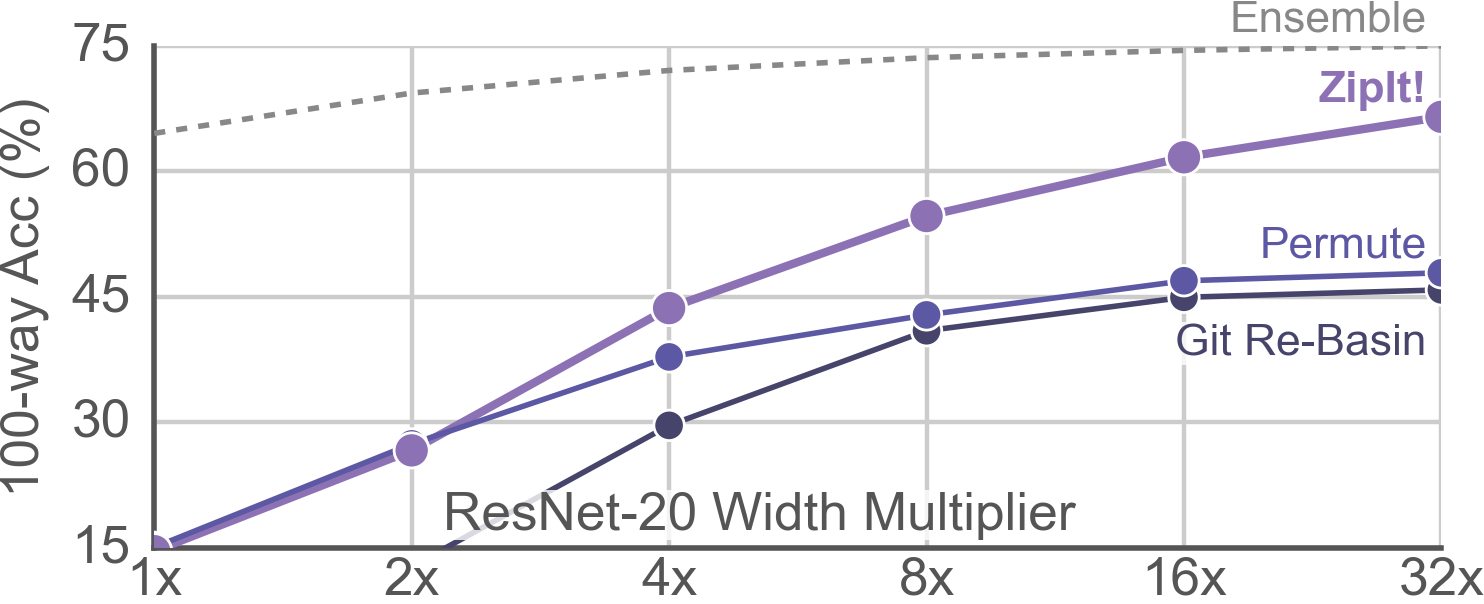
\includegraphics[width=0.95\linewidth]{figures/imgs/model_scale.png}
%         \caption{{\bf Model Scale.} As we increase the width of the ResNet-20 models used for the CIFAR-100 (50+50) setting, \name{}\ makes effective use of that extra capacity, quickly approaching ensemble accuracy. 
%         Git Re-Basin \cite{ainsworth2022git} and Permute only slightly benefit from the extra scale.
%         }
%         \label{fig:model_size}
%         % \vspace{-60pt}
%     \end{minipage}
% }\end{minipage}
% \end{wrapfigure}